\chapter{User Interface}
\begin{figure}[h!]
	\centering
	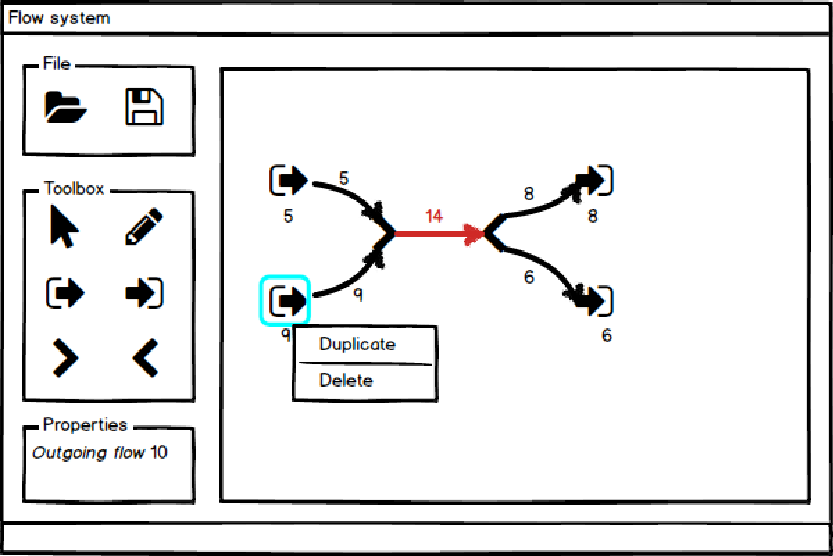
\includegraphics{figures/mockup.pdf}
	\caption{Mockup}
	\label{fig:mockup}
\end{figure}

\section{Specifications}

\begin{tabularx}{\textwidth}{|p{2cm}X|}\hline
	Code & Specification \\\hline
	UIS-010 & An open file dialog box will be showed by pressing \faicon{folder-open}. \\\hline
	UIS-020 & A save file dialog box will be showed by pressing \faicon{floppy-o}. \\\hline
	UIS-030 & The sidebar contains a toolbox. \\\hline
	UIS-030A & The application has different modes, only one button can be selected in the toolbox.  \\\hline
	UIS-040 & The normal mode is selected by default \faicon{mouse-pointer}. \\\hline
	UIS-040A & In normal mode a component can be selected by clicking on it. \\\hline
	UIS-040B & A selected item is outlined and the properties can be changed in the properties window. \\\hline
	UIS-040C & A selected item can be moved by dragging. \\\hline
	UIS-040D & In normal mode a context-menu appears when pressing right-click on a component which gives the following options to the component: duplicate and delete. \\\hline
	UIS-050 & The draw mode can be selected by pressing \faicon{pencil}. \\\hline
	UIS-050A & The draw mode allows to draw a pipeline between an unused output of a component to an unused input of another component. \\\hline
	UIS-060 & A pump can be added to the network by selecting \faicon{sign-out} and then the drawing. \\\hline
	UIS-070 & A sink can be added to the network by selecting \faicon{sign-in} and then the drawing. \\\hline
	UIS-080 & A merger can be added to the network by selecting \faicon{chevron-right} and then the drawing. \\\hline
	UIS-090 & A splitter can be added to the network by selecting \faicon{chevron-left} and then the drawing. \\\hline
	UIS-100 & After a component is added to the flow network the mode is set back to normal. \\\hline
	UIS-110 & The sidebar has a properties box which allows to edit the properties of the a selected component. \\\hline
	UIS-120 & The flow network is shown in the drawing. \\\hline
	UIS-130 & Each component displays the current flow except for splitter and merger. \\\hline
	UIS-140 & Components that have missing connectors on the input or output are displayed in orange. \\\hline
	UIS-150 & Pipelines that exceed the maximum flow are shown in red.\\\hline
\end{tabularx}